\documentclass[11pt]{opticajnl}
\journal{opticajournal} % use for journal or Optica Open submissions

% See template introduction for guidance on setting shortarticle option
\setboolean{shortarticle}{true}
% true = letter/tutorial
% false = research/review article

% ONLY applicable for journal submission shortarticle types:
% When \setboolean{shortarticle}{true}
% then \setboolean{memo}{true} will print "Memorandum" on title page header
% Otherwise header will remain as "Letter"
% \setboolean{memo}{true}
\usepackage{lineno}
\usepackage{listings}
\usepackage{xcolor}  % Para colorear el código

% Definir colores para la sintaxis de Python
\definecolor{pystring}{RGB}{186,33,33}      % Strings
\definecolor{pycomment}{RGB}{107,107,107}   % Comentarios
\definecolor{pykeyword}{RGB}{0,119,170}     % Palabras clave
\definecolor{pybuiltin}{RGB}{163,21,21}     % Funciones builtin
\definecolor{pybackground}{RGB}{250,250,250} % Fondo

% Definir el estilo para código Python
\lstdefinestyle{Python}{
    language=Python,
    backgroundcolor=\color{pybackground},
    basicstyle=\ttfamily\small,
    breakatwhitespace=false,
    breaklines=true,
    captionpos=b,
    keepspaces=true,
    numbers=left,
    numbersep=5pt,
    showspaces=false,
    showstringspaces=false,
    showtabs=false,
    tabsize=4,
    frame=single,
    commentstyle=\color{pycomment},
    keywordstyle=\color{pykeyword},
    stringstyle=\color{pystring},
    identifierstyle=\color{black},
    numberstyle=\tiny\color{gray},
    emphstyle=\color{pybuiltin},
    morekeywords={import,from,as,def,class,return,yield,for,while,if,else,elif,
                  try,except,finally,with,lambda,assert,pass,break,continue,
                  raise,global,nonlocal,True,False,None,and,or,not,is,in},
    emph={pandas,numpy,matplotlib,seaborn,sklearn,tensorflow,torch,
          plt,pd,np,sns,print,len,range,enumerate,zip,dict,list,tuple,set,
          min,max,sum,sorted,map,filter},
}

\lstdefinestyle{sql}{
  language=SQL,
  showspaces=false, 
  basicstyle=\ttfamily,
  numbers=left,
  numberstyle=\tiny,
  backgroundcolor=\color{gray!10},
  keywordstyle=\color{blue}\bfseries,
  commentstyle=\color{green!70}\ttfamily,
  stringstyle=\color{red!70}\ttfamily,
  breaklines=true,
  morekeywords={CREATE, DROP, TABLE, SELECT, INSERT, UPDATE, DELETE, FROM, WHERE, JOIN, ON, AS}, % Puedes añadir más palabras clave específicas de SQL.
  literate={``}{``}1 {''}{''}1 {“}{``}1 {”}{''}1 {‘}{`}1 {’}{'}1
}

\lstdefinestyle{terminal}{
  backgroundcolor=\color{white},   % Fondo blanco
  basicstyle=\color{black}\ttfamily, % Texto negro en fuente monoespaciada
  keywordstyle=\color{blue}\bfseries, % Palabras clave en azul y negrita
  commentstyle=\color{green!70}\ttfamily, % Comentarios en verde
  stringstyle=\color{red}\ttfamily, % Cadenas en rojo
  morekeywords={sudo, apt-get, install, cd, ls, mkdir, rm, rmdir, cp, mv, echo, cat, nano, vim, grep, find, chmod, chown, systemctl, service, update, upgrade, reboot, shutdown, exit}, % Comandos comunes de terminal
  breaklines=true, % Permitir saltos de línea
  frame=single, % Marco alrededor del código
  framerule=0.5pt, % Grosor del marco
  rulecolor=\color{gray}, % Color del marco
  xleftmargin=0.05\textwidth, % Margen izquierdo
  xrightmargin=0.05\textwidth, % Margen derecho
  aboveskip=1em, % Espacio antes del bloque de código
  belowskip=1em % Espacio después del bloque de código
}
\definecolor{rstring}{RGB}{186,33,33}     % Strings
\definecolor{rcomment}{RGB}{0,128,0}      % Comentarios
\definecolor{rfunction}{RGB}{0,0,255}      % Funciones
\definecolor{rkeyword}{RGB}{145,0,145}    % Palabras clave
\definecolor{rbackground}{RGB}{248,248,248} % Fondo

\lstdefinestyle{R}{
    language=R,
    backgroundcolor=\color{rbackground},
    basicstyle=\ttfamily\small,
    breakatwhitespace=false,
    breaklines=true,
    captionpos=b,
    keepspaces=true,
    numbers=left,
    numbersep=5pt,
    showspaces=false,
    showstringspaces=false,
    showtabs=false,
    tabsize=2,
    frame=single,
    commentstyle=\color{rcomment},
    keywordstyle=\color{rkeyword},
    stringstyle=\color{rstring},
    identifierstyle=\color{black},
    numberstyle=\tiny\color{gray},
    morekeywords={library, data.frame, read.csv, ggplot, aes, geom_bar, theme_minimal, 
                  scale_fill_manual, gather, group_by, summarise, arrange, filter},
}


%\linenumbers % Turn off line numbering for Optica Open preprint submissions.

\title{Cuadros de mando}

\author[1,2,3]{Luis Ardévol Mesa}


\begin{abstract}
Buscamos un cuadro de mando con 4 paneles que muestre el director (o combinaciones de directores) con mayor ROI promedio, y las productoras con mayor cuota de mercado en el año 2001. Además, se mostrarán \textit{rankings} de directores y productoras mejor valorados. Se proporcionan consultas SQL y MDX para obtener estos datos, así como distintas visualizaciones del cuadro de mando.
\end{abstract}

\setboolean{displaycopyright}{false} % Do not include copyright or licensing information in submission.

\begin{document}

\maketitle

En caso de no copiarse correctamente el código SQL o MDX, se pueden encontrar las consultas en el archivo \texttt{README} adjunto.

 
\section{Consultas}

\subsection{Consulta SQL que obtiene un ranking directores}

\begin{lstlisting}[style=terminal]
select d.nombre as director, cast(avg(su.satisfaccion) as numeric(2,1)) as valoracion, sum(su.votos) as votos
from public.satisfaccion_usuarios su, public.tiempo t, public.director d
where su.director = d.id
	and su.tiempo_emision = t.id
group by d.id
order by valoracion desc
\end{lstlisting}

\subsection{Consulta MDX para el ROI promedio por director/es}

\begin{lstlisting}[style=terminal]
WITH
  MEMBER [Measures].[roiPromedio] AS
    ([Measures].[beneficio] / [Measures].[coste])
SET [~ROWS_director_director.jerarquiadirector] AS
    {[director.jerarquiadirector].[niveldirector].Members} -- Solo directores
SELECT
  NON EMPTY {[Measures].[roiPromedio]} ON COLUMNS,
  NON EMPTY TopCount(
    [~ROWS_director_director.jerarquiadirector], 
    30, 
    [Measures].[roiPromedio]
  ) ON ROWS
FROM [finanzas]
\end{lstlisting}
\newpage
\subsection{Consulta SQL que obtiene un ranking de productoras}

\begin{lstlisting}[style=terminal]
select p.nombre as productora, cast(avg(su.satisfaccion) as numeric(2,1)) as valoracion, sum(su.votos) as votos
from public.satisfaccion_usuarios su, public.tiempo t, public.productora p
where su.productora = p.id
	and su.tiempo_emision = t.id
	and position(',' in p.nombre) = 0
group by p.id
order by valoracion desc
\end{lstlisting}

\subsection{Consulta MDX para la cuota de mercado de las productoras en 2001}

\begin{lstlisting}[style=terminal]
WITH
  MEMBER [Measures].[cuotaMercado] AS
    ((100 * [Measures].[ingresos]) / 
      Sum([productora].[nivelproductora].Members, [Measures].[ingresos]))
SET [~ROWS_productora_productora.jerarquiaproductora] AS
    {[productora.jerarquiaproductora].[nivelproductora].Members}
SET [~ROWS_tiempoemision_tiempoemision.jerarquiatiempo] AS
    {[tiempoemision.jerarquiatiempo].[anno].[2001]}
SELECT
  NON EMPTY {[Measures].[cuotaMercado]} ON COLUMNS,
  NON EMPTY TopCount(
    NonEmptyCrossJoin(
      [~ROWS_productora_productora.jerarquiaproductora], 
      [~ROWS_tiempoemision_tiempoemision.jerarquiatiempo]
    ), 
    10, 
    [Measures].[ingresos]
  ) ON ROWS
FROM [finanzas]
\end{lstlisting}



\section{Visualizaciones}

\begin{figure}[H]
\centering
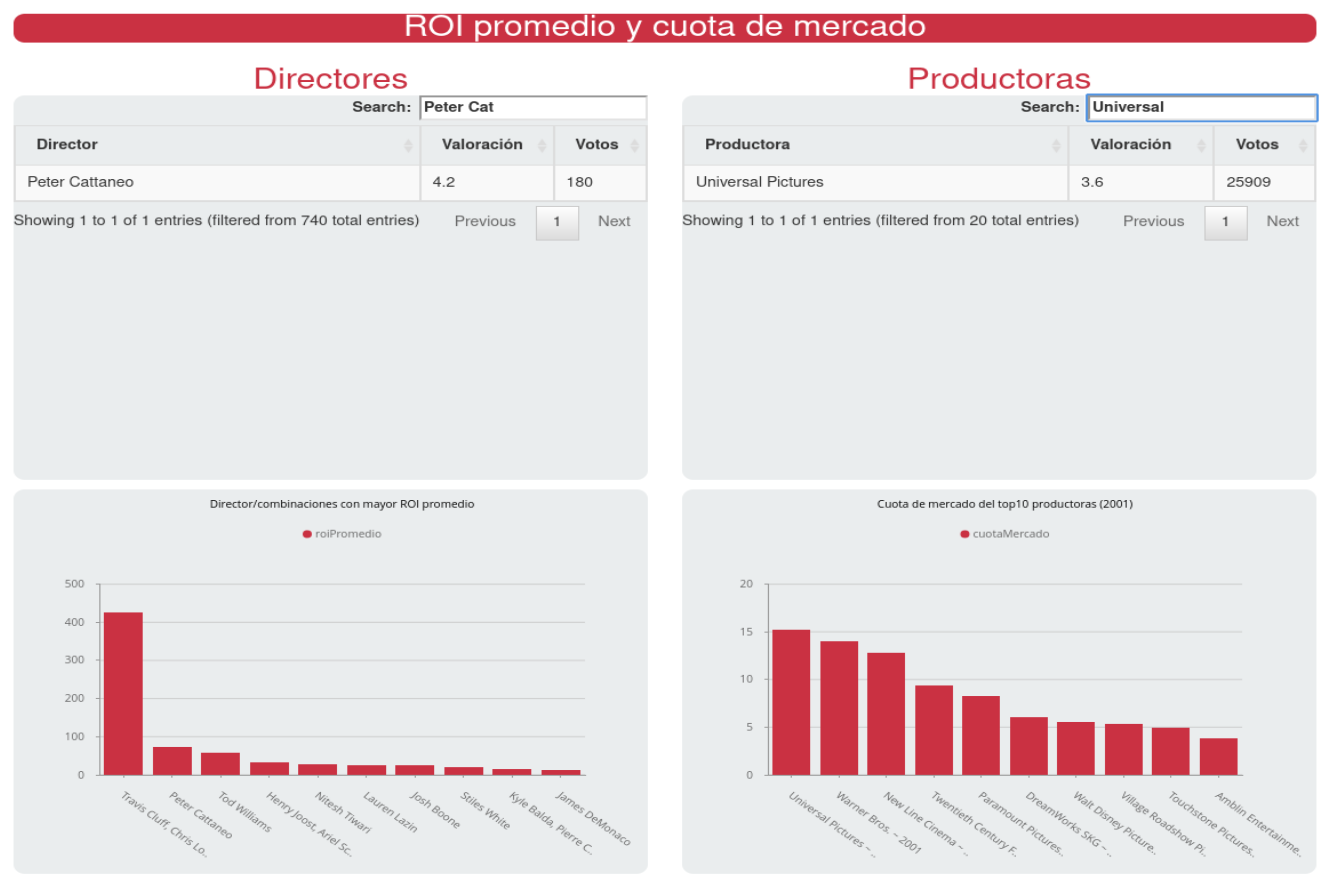
\includegraphics[width=0.8\textwidth]{fotos/1.png}
\caption{Filtramos por Peter Cattaneo, segundo director con mayor ROI promedio y una valoración promedio de 4.2 sobre 5. Filtramos la valoración de la productor con mayor cuota de mercado en 2001.}
\end{figure}

\begin{figure}[H]
\centering
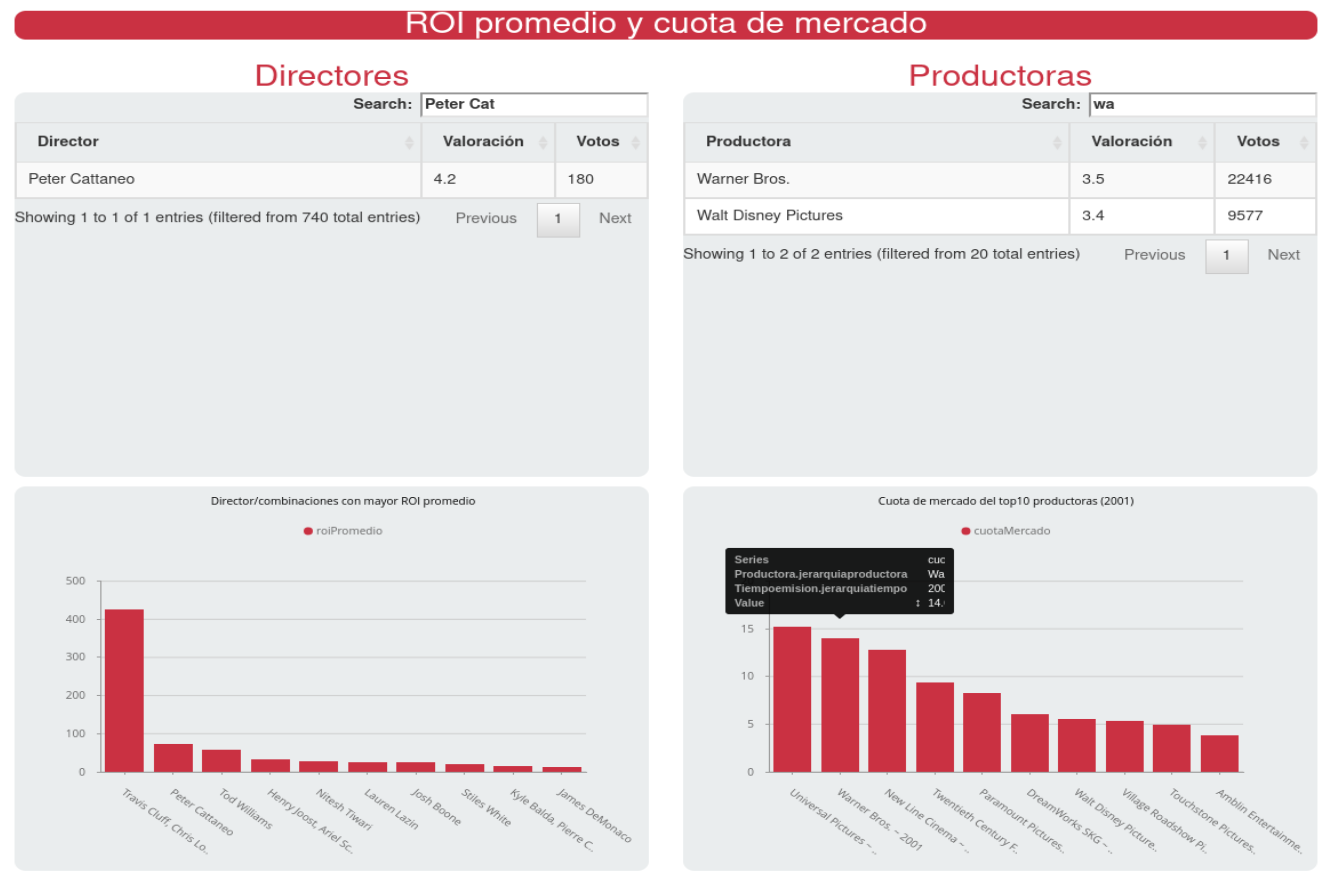
\includegraphics[width=0.8\textwidth]{fotos/2.png}
\caption{Mostramos la valoración de Warner Bros (junto con su cuota de mercado en 2001) y Walt Disney Pictures.}
\end{figure}

\begin{figure}[H]
\centering
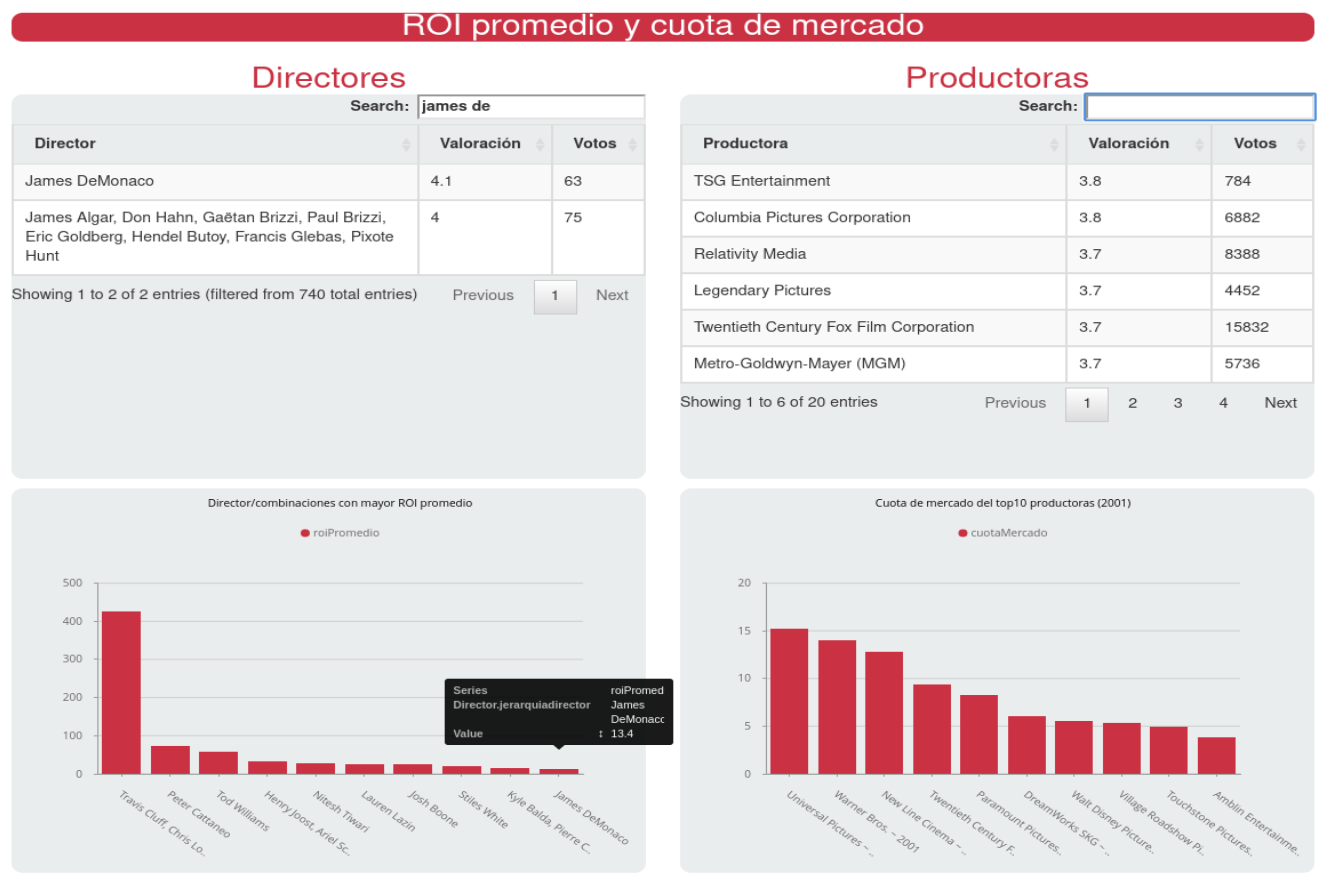
\includegraphics[width=0.8\textwidth]{fotos/3.png}
\caption{Estudiamos la valoración promedio del último director mostrado en la gráfica de mayor ROI promedio, James DeMonaco.}
\end{figure}

\begin{figure}[H]
\centering
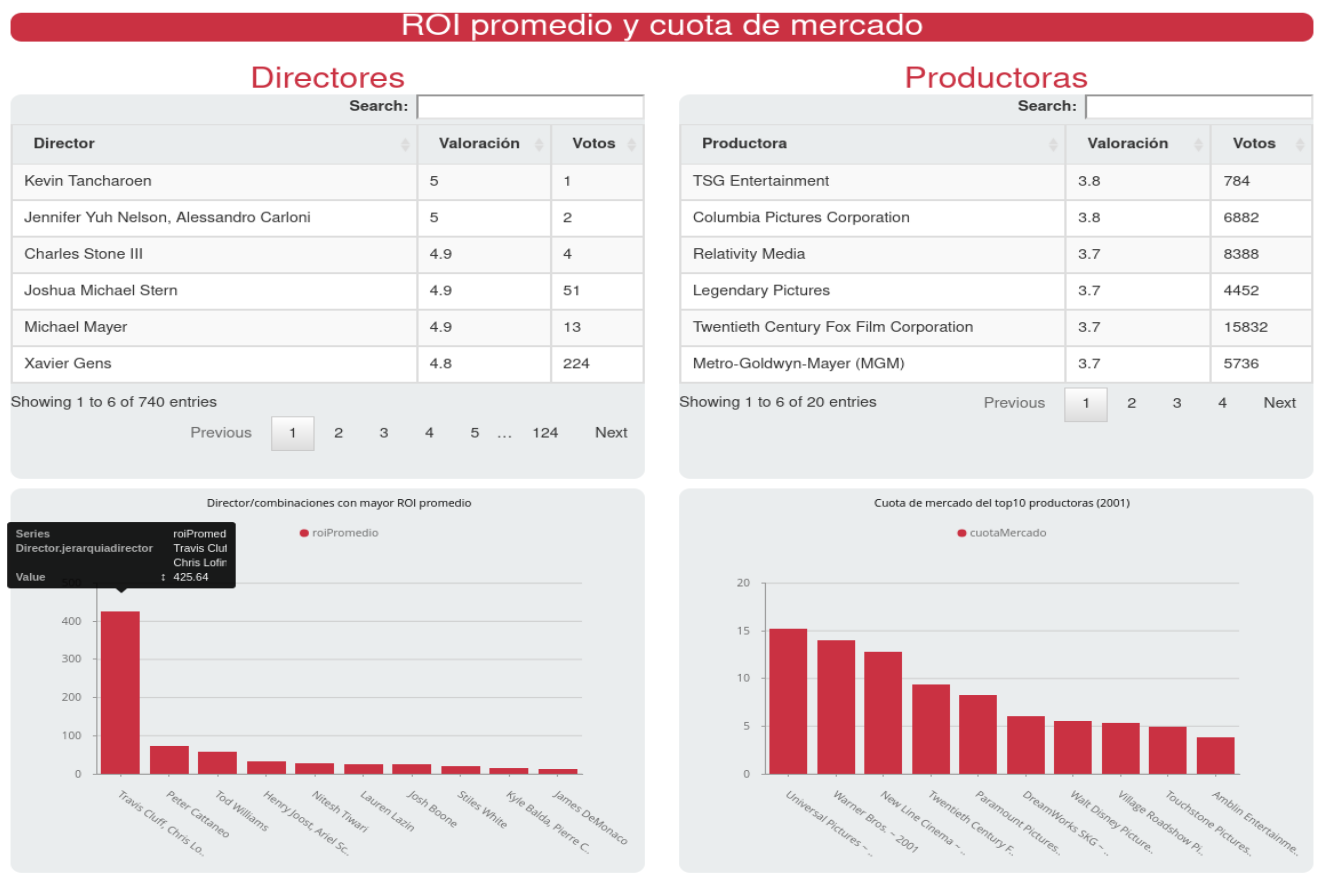
\includegraphics[width=0.8\textwidth]{fotos/5.png}
\caption{Mostramos las estadísticas de la combinación de directores con mayor ROI promedio.}
\end{figure}

\begin{figure}[H]
\centering
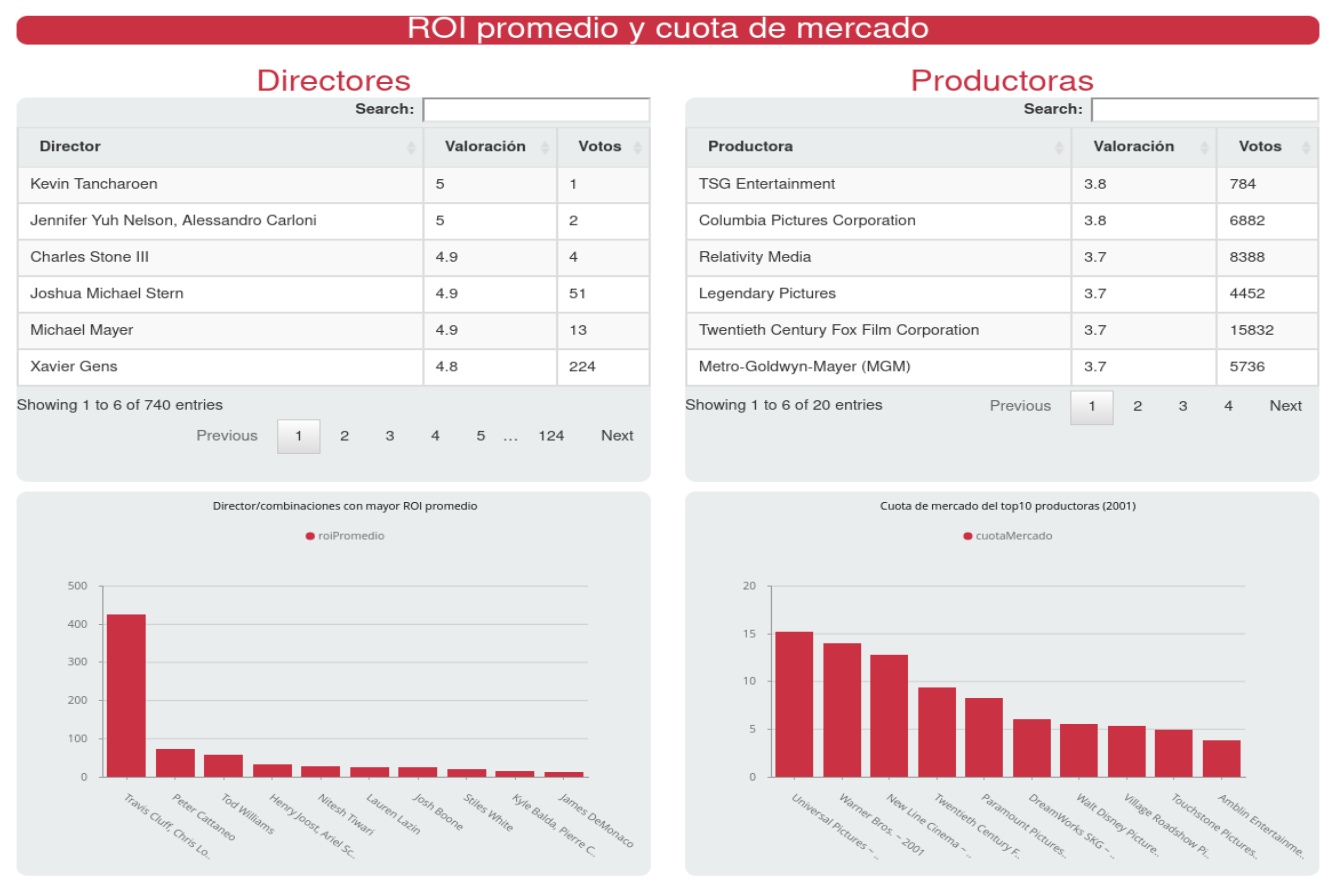
\includegraphics[width=0.8\textwidth]{fotos/4.png}
\caption{Mostramos el cuadro de mando sin ningún tipo de filtro.}
\end{figure}

\end{document}
